\section{Interactive System}


%\begin{figure}[ht]
%\centering
%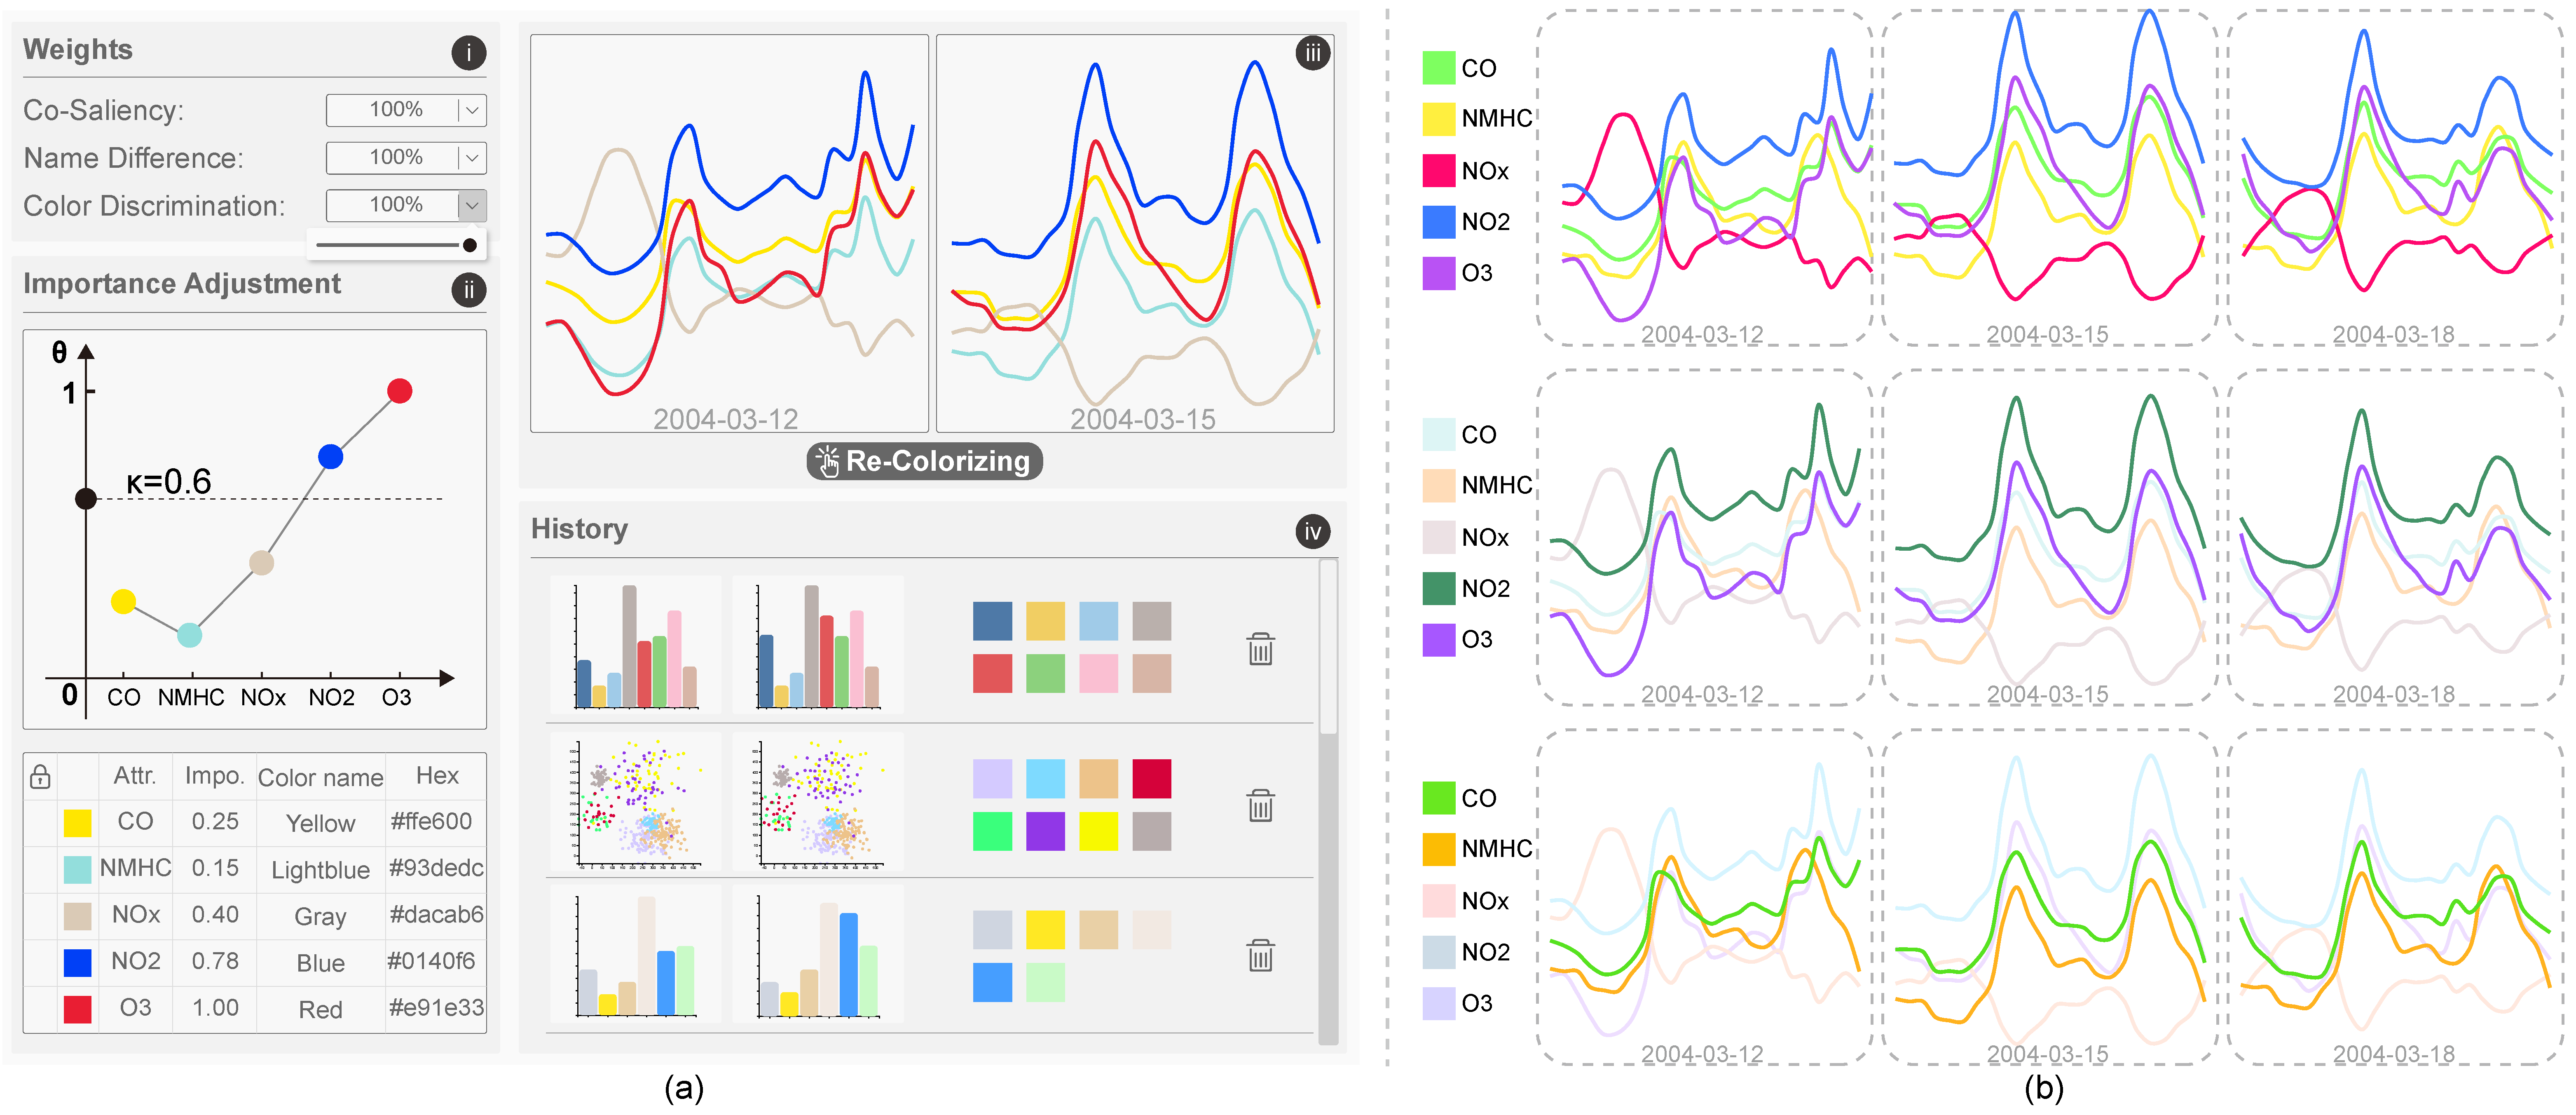
\includegraphics[width=0.8\columnwidth]{figures/interface.pdf}
%\caption{Screenshot of the interactive system. (a) Settings Panel; (b) Control Panel; (c) Visualization Panel; (d) History Panel.}
%\vspace*{-3mm}
%\label{fig:ui}
%\end{figure}

%\subsection{Interactive System}
\label{sec:interaction}
To help users interactively design colors for comparing multi-class scatterplots, we developed a web-based multi-view visualization tool \footnote{\small \url{https://c3-palette.github.io/}}.
The screenshot of the interface can be found in the supplemental material.
This tool consists of four coordinated views: (a) a settings panel, (b) a control panel for adjusting importance threshold $\kappa$ and even importance value of each class, (c) the juxtaposed visualizations, and (d) a history view. The control panel shows the decision which classes are highlighted, and the history view allows to quickly explore and access previous color mappings.

After uploading multiple categorical scatterplots, the user can either choose a default color palette or use our system to automatically generate color palettes. In this case, the system automatically finds an optimal color mapping scheme to colorize the input data, while each class is encoded as a circle where the x-axis represents class label and the y-axis indicates the importance of each class. By default, the importance is represented by the change degree and $\kappa$ is set to zero. User can drag the circle to modify the corresponding importance value. The $\kappa$ is controlled by a black circle on the y-axis which can also be dragged to modify. Our system finds a color mapping scheme to highlight the classes with large importance and renders the classes in ascending order of the corresponding importance. If users like the color mapping scheme, they can save it to the history view.




\subsection{Case Study}
\label{sec:caseStudy}


\begin{figure}[!t]
\centering
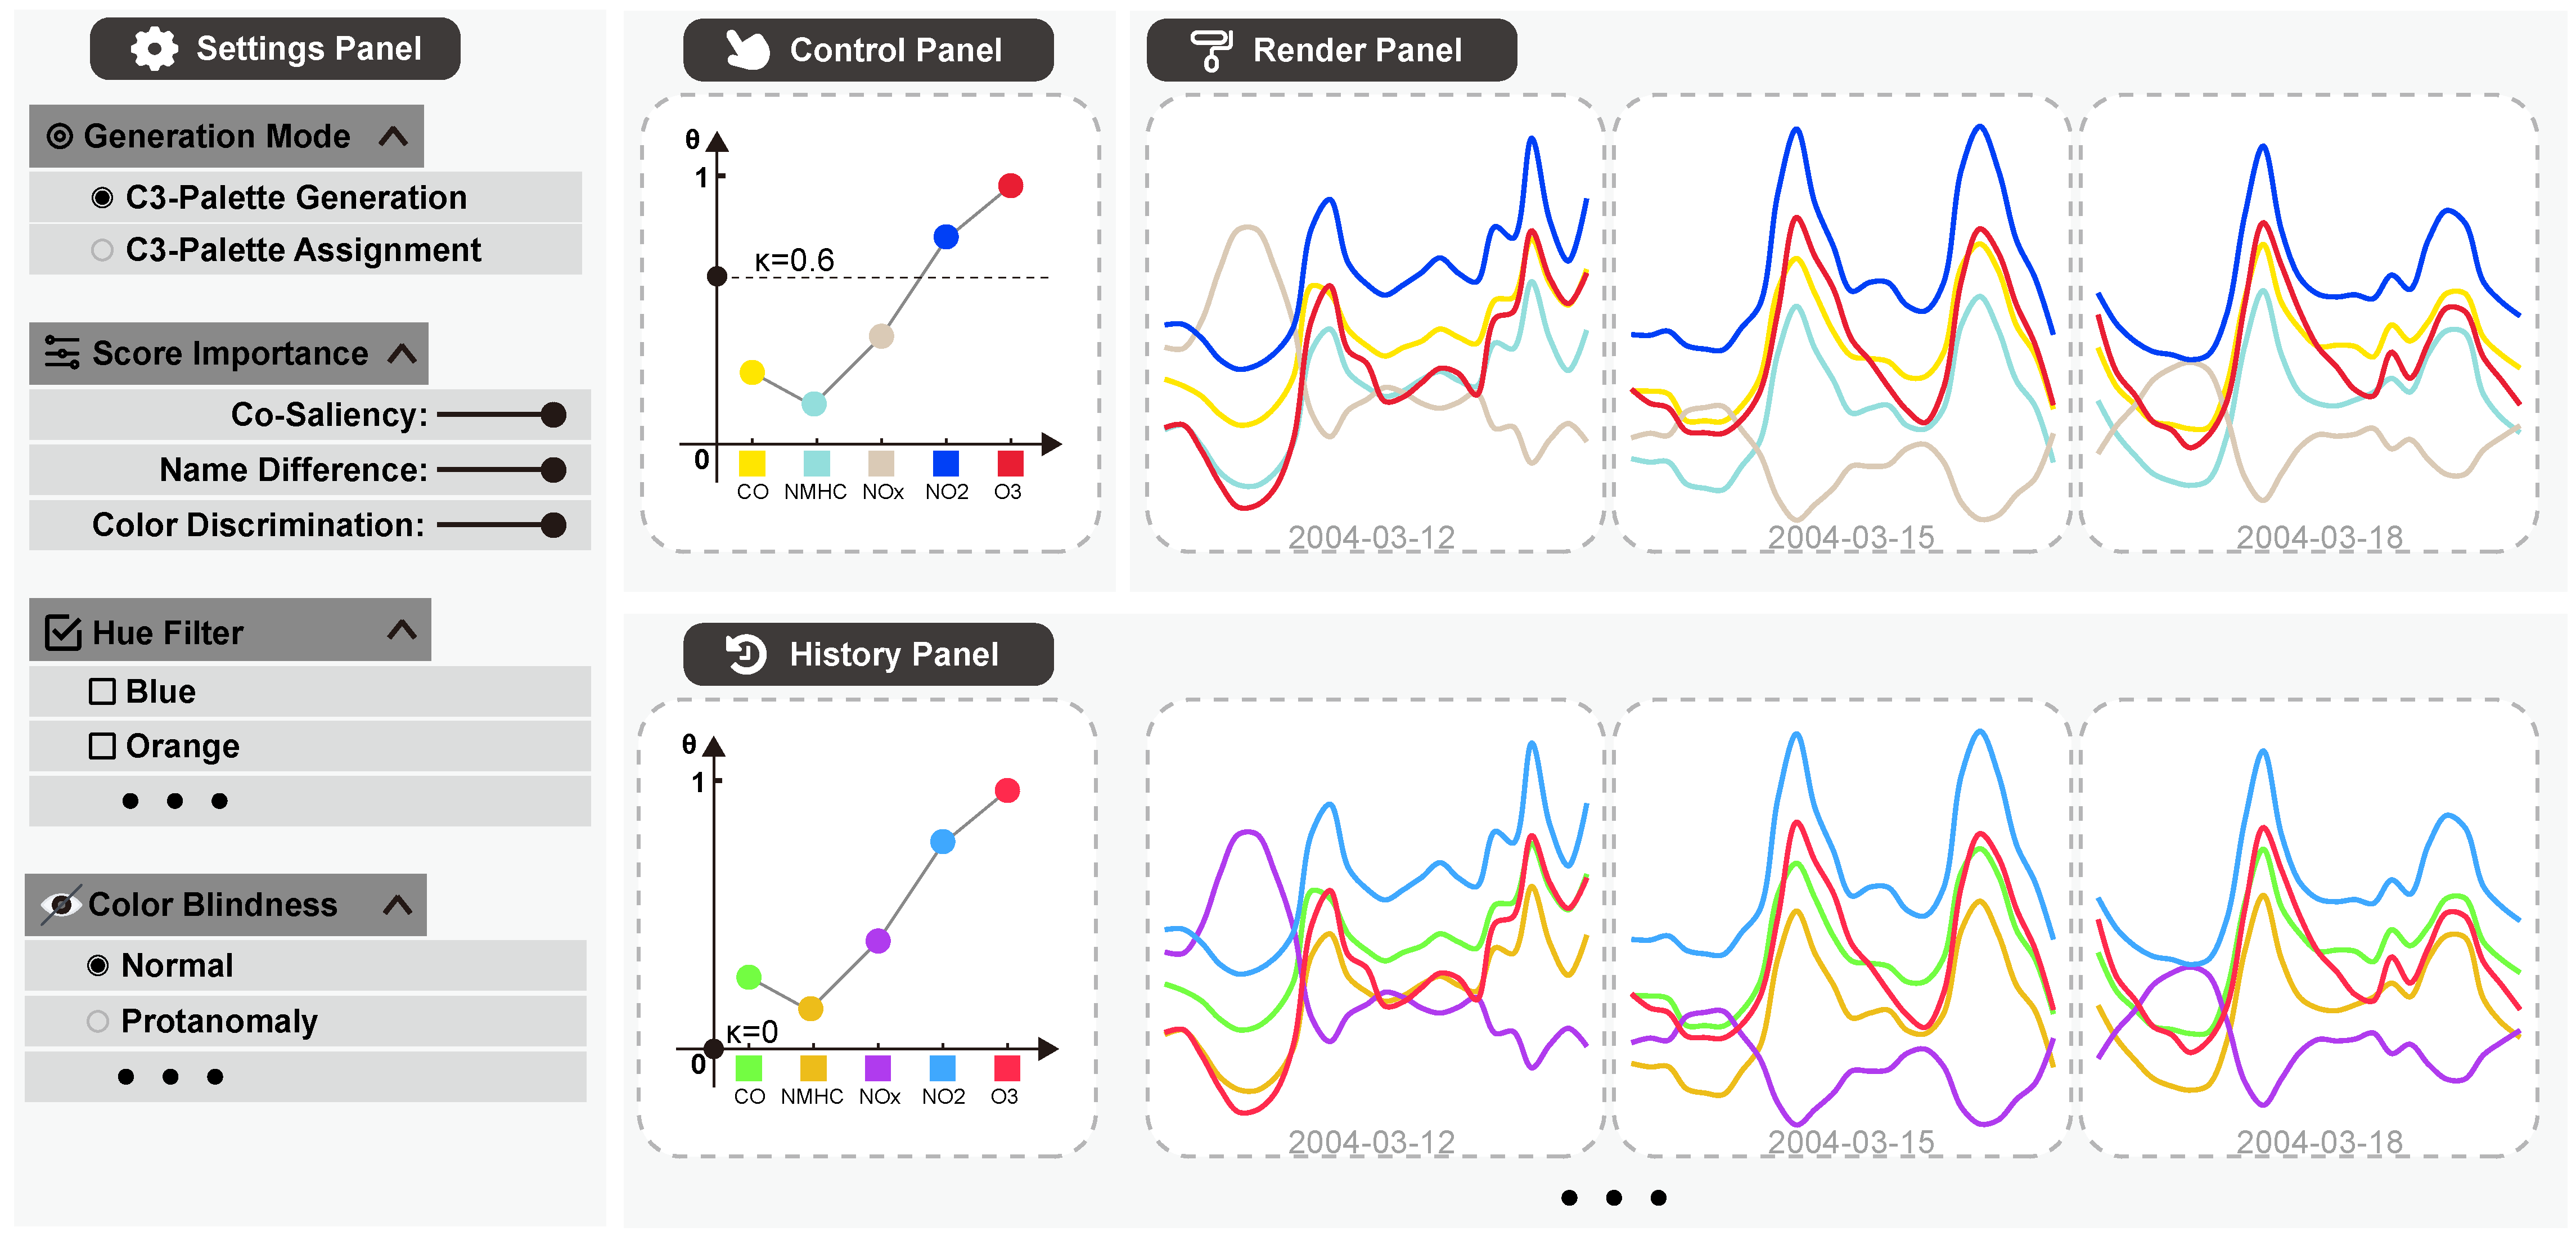
\includegraphics[width=1\linewidth]{figures/case-linechart-2.pdf}
\caption{Exploring the changes of gases in an air quality data set~\cite{DEVITO2008750}. (a) The automatic generated palette creates salient colors for  all lines. (b) Two selected lines are popping out from the other lines in three views.}
\vspace*{-3mm}
\label{fig:caseStudy2}
\end{figure}

To shed further light onto the ecological validity of our approach, we conducted a case study on a real-world categorical dataset visualized with line charts.
Here, we analyze an air quality data set ~\cite{DEVITO2008750} that contains hourly responses of a gas multi-sensor device deployed in an Italian city from March 12 to March 18, 2014.
Fig.~\ref{fig:caseStudy2} shows the juxtaposed line graphs encoded by our generated color palette, where each gas type is represented by a line with a unique color.
We can see that all gases are encoded with highly salient colors, making it hard to explore changes of specific gases. This is reasonable because the default $\kappa$ is zero, but all gases have large changes.
Thanks to our interaction mechanism, users can directly select classes of interest to be highlighted,  the $f(\theta)$ values of the other classes are then automatically set to -1. Using the hue-preserving palette generation method, the produced palette lets the selected lines pop out from the others (see Fig.~\ref{fig:caseStudy2}(b)). Hence, users can easily explore the changes of the selected two gases (NO$_2$ and O$_3$) in the three juxtaposed views.


